\section{Evaluation and Results}
\label{sec:results}

\begin{table}[]
    \caption{Number of automated daily requests towards web applications compared to the number of unique entry points.}
    \centering
    \begin{tabular}{|l|l|l|}
    \hline
    \textbf{Web Application} & \textbf{Requests/Day} & \textbf{Unique Endpoints} \\ \hline
    WordPress                & 558,576               & 152 (99.97\% $\blacktriangledown$)             \\ \hline
    phpMyAdmin               & 491,400               & 107 (99.98\% $\blacktriangledown$)             \\ \hline
    HotCRP                   & 175,848                 & 32 (99.98\% $\blacktriangledown$)              \\ \hline
    FluxBB                   & 63,624                & 17 (99.97\% $\blacktriangledown$)              \\ \hline
    \end{tabular}
    \label{tab:logreduction}
\end{table}

In this section, we employ \animatedead{} to debloat web applications. 
We start by collecting the list of entry points exercised while using popular web applications. 
We then configure \animatedead{} to explore feasible paths from those entry points. 
The result of this step is a list of exercised modules in target web applications. 
These modules are reachable from the list of entry points. 
Then, by removing the unused modules, we produce debloated web applications. 
In the remainder of this section, unless mentioned otherwise, we discuss the results of function debloating (i.e., removing functions with no callers) as it strictly outperforms file debloating.

Debloating based on concolic execution in \animatedead{} has multiple benefits over the previously explored dynamic debloating schemes that rely on runtime tracing to collect code-coverage information from users:

\begin{itemize}
    \item By relying on existing logging mechanism of web servers, we can collect usage traces for long periods of time for web applications with a large user base with small overhead.
    \item By analyzing each entry point in an abstract state (i.e., abstract request parameters, database, and network requests), the resulting code-coverage incorporates the functionality for all actions that are possible through each entry point and all possible database and network responses (i.e., including successful and failure cases), resulting in robust debloated applications (Section~\ref{sec:automated_random_testing}). 
\end{itemize}

\subsection{Experimental Setup}

In our evaluation, we focus on four popular web applications with different size and functionality. 
Our dataset includes phpMyAdmin 4.7 (database administration), WordPress 4.6.22 (content management system), HotCRP 3.0 (submission management), and FluxBB 1.5.11 (online forum platform). 

We run our analysis using 20 worker nodes (running \animatedead{}'s PHP emulator), and 5 orchestrators running inside Docker on an Ubuntu 22.04 LTS host with 20 CPU cores and 32GB of memory. 
For each web application, we follow their installation steps to generate the configuration files. 
This step is necessary as \emph{all} web applications in our dataset verify the presence of configuration files (e.g., \texttt{wp-config.php} for WordPress) and redirect user requests to the installation page if the post-installation files are absent from the file system. 

We configured concolic execution campaigns with the threshold of 24 hours, though in practice, the majority of entry points converge to their maximum code-coverage in less than one hour. 
Analysts can observe the progress made by \animatedead{} through the reporting panel and decide to terminate the analysis when \animatedead{} stops identifying new code-coverage or the queue becomes empty (i.e., all paths for an entry point are explored). 

\begin{figure*}[t]
    \centering
    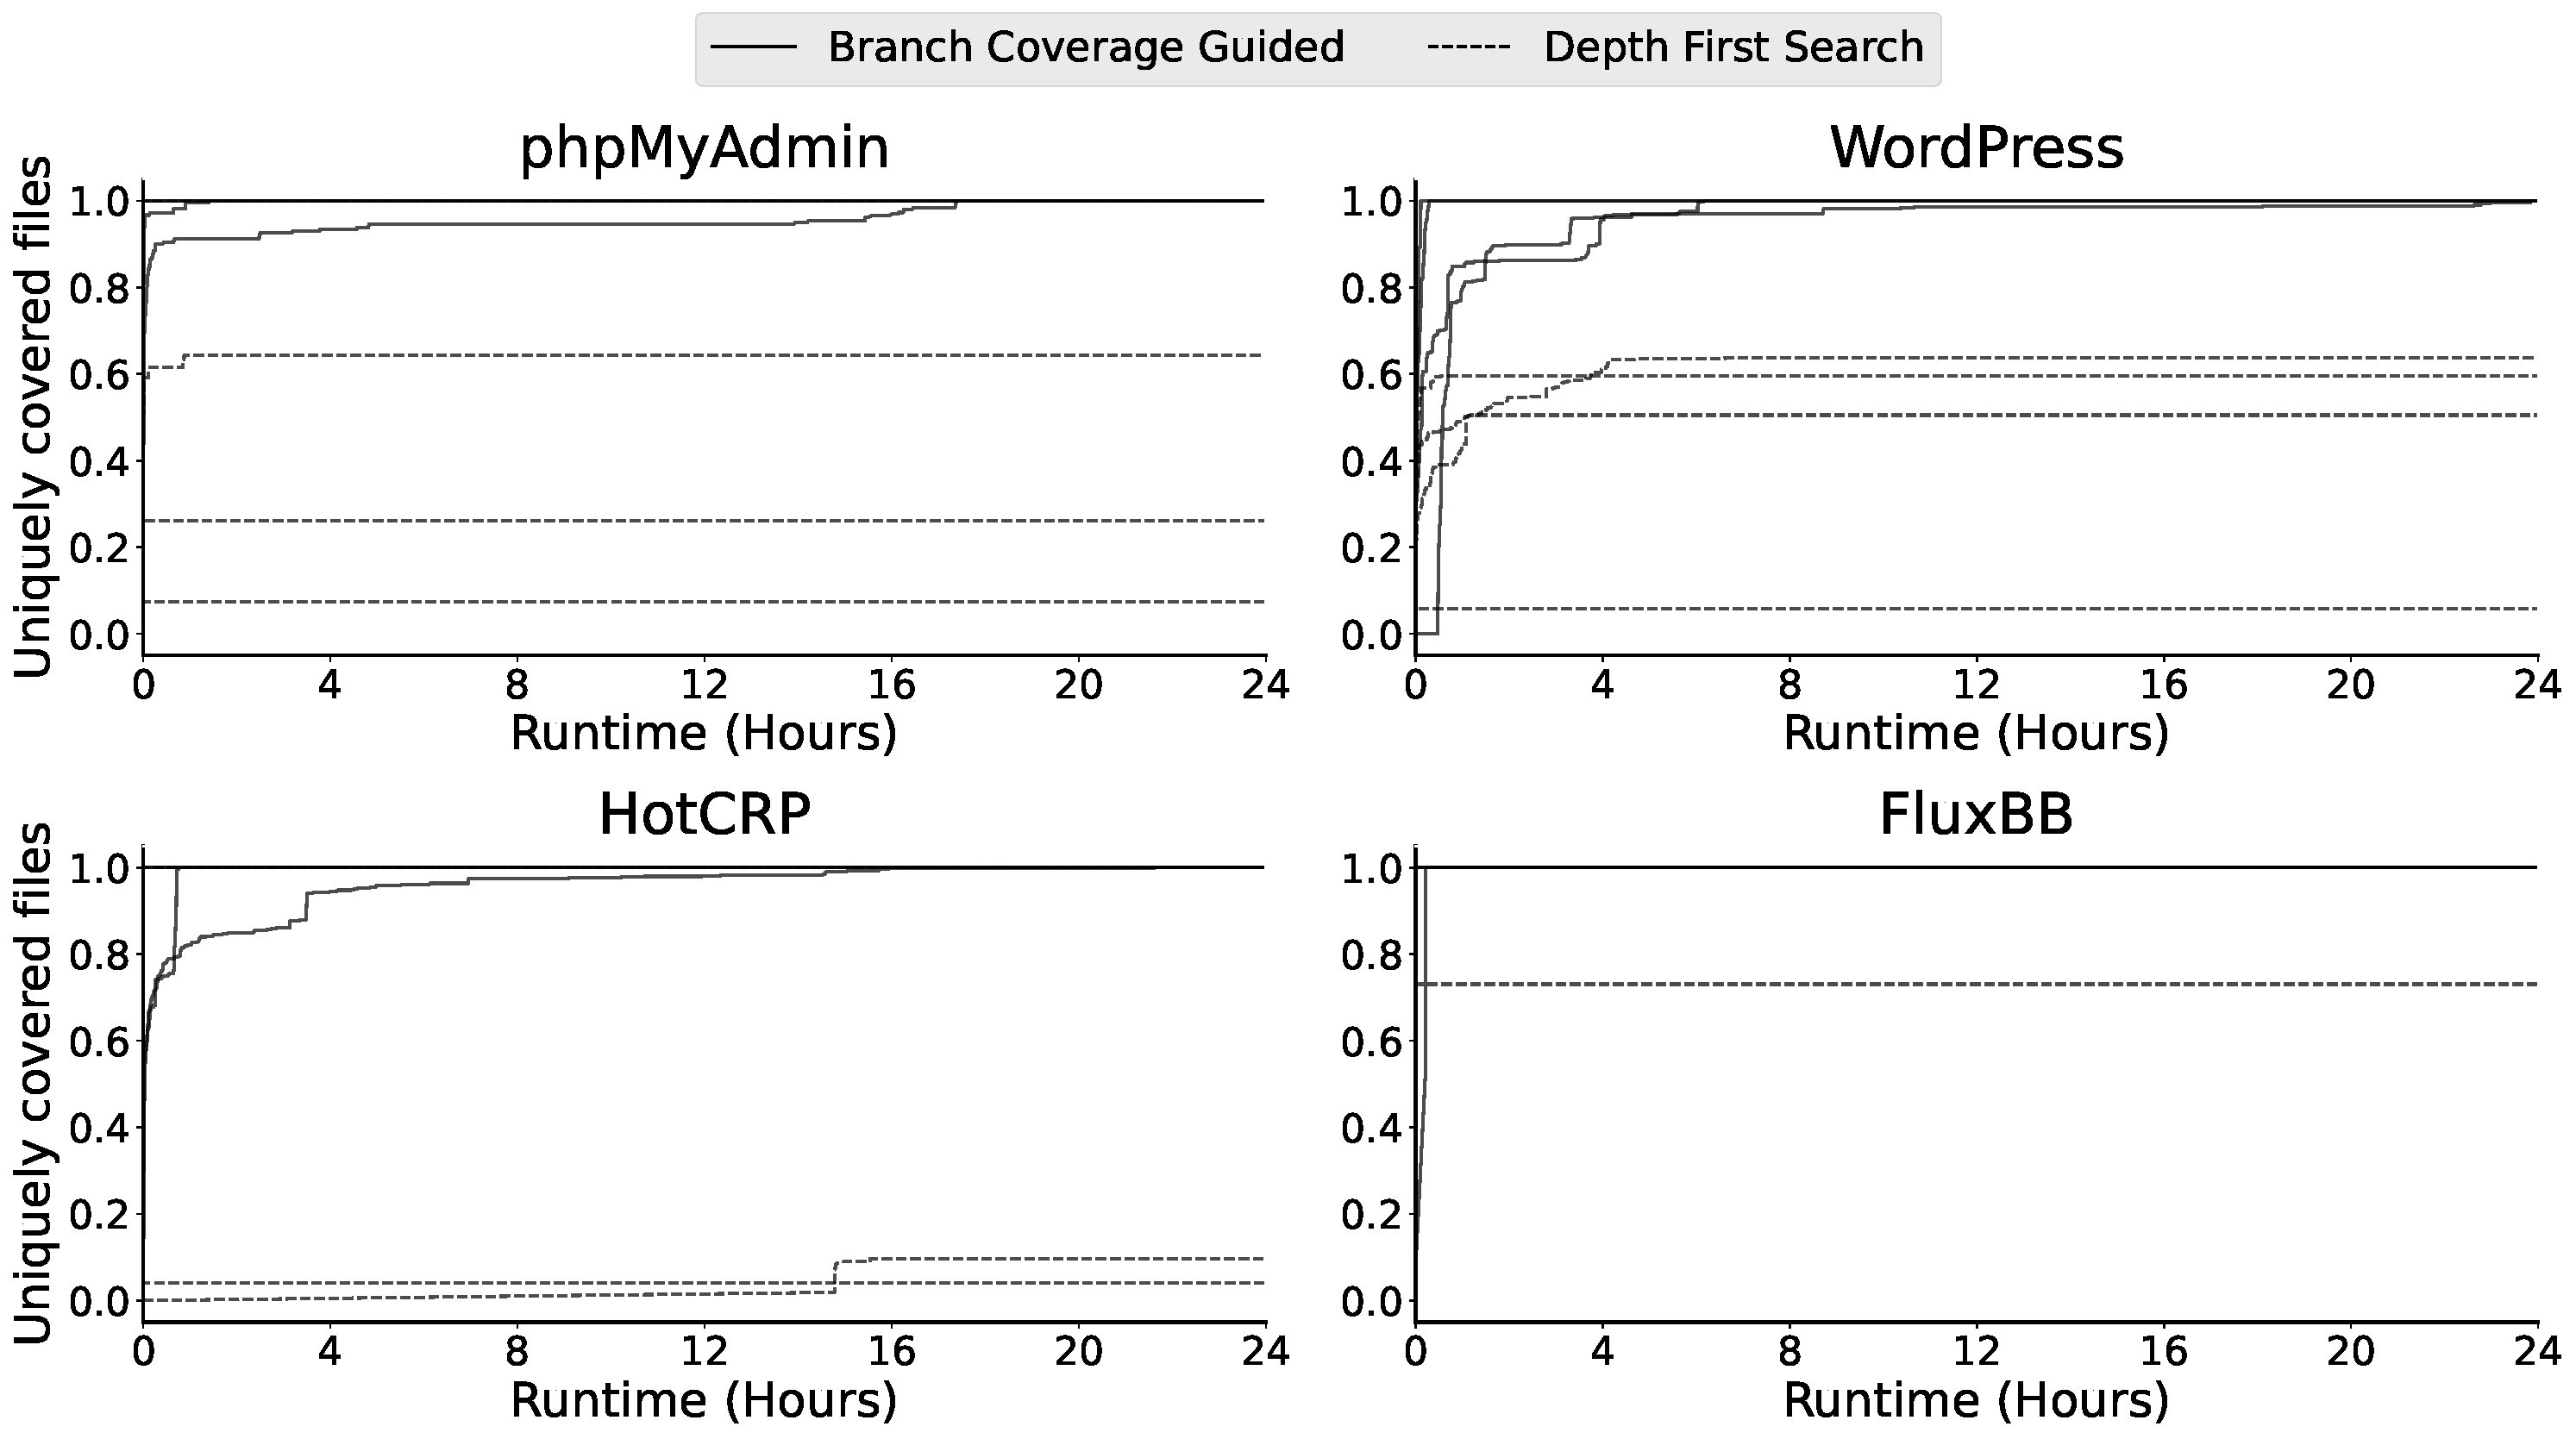
\includegraphics[width=\textwidth]{figures/ad/execution_convergence_2rows.pdf}
    \caption{Unique files discovered over time using DFS and Branch coverage guided path prioritization. Branch coverage approach results in a higher number of discovered files while DFS gets stuck in the same parts of the code.}
    \label{fig:execution_convergence}
\end{figure*}

\subsubsection*{Data Collection} 
To compare the debloating performance of \animatedead{} with prior work and to generate baseline code-coverage information for each entry point, we rely on the automated tests provided by the ``Less is More''~\cite{azad2019less}. 

We run the Selenium scripts from Less is More and the ones we built for HotCRP and FluxBB and collect the web server logs along with the dynamic code-coverage information from the Less is More framework. 
The code-coverage information for our web applications serves as the baseline code-coverage (i.e., dynamic code-coverage) for the remainder of our evaluation. 

We expect the resulting code-coverage of \animatedead{} to be a superset of the dynamic code-coverage information. 
Any file or function covered in the dynamic code-coverage that is missed by \animatedead{} would signify a false positive (i.e., removal of a feature that is required by users). 

\subsubsection*{Data Cleaning and Summarization} 
It is common for popular entry points (e.g., \texttt{index.php}) of web applications to receive a large number of requests. 
To prevent our tool from performing the same analysis multiple times unnecessarily, we only retain unique entry points and parameters from the web server logs. 

In the initial stages of the analysis, \animatedead{} removes duplicate log entries. 
Since we analyze the application with an abstract database, different values for the same parameters will have a similar effect (e.g., \texttt{?page\_id=1} or {\texttt{2}). 
This deduplication also shrinks the total number of entry points significantly. 
Table~\ref{tab:logreduction} lists the total number of log entry points produced over a 24 hour period by running the automated tests (Selenium, and crawler) repeatedly (simulating different users of a web application exercising the same functionality), compared to the final number of unique entries used by \animatedead{} for analysis. 
Across all web applications in our dataset, we observe a reduction of over 99.9\% in the number of unique entries to be analyzed. 
Moreover, web applications with a smaller code-base (i.e., FluxBB and HotCRP) produce fewer unique entry points. 

\subsection{Generating the Code-coverage}

We take the logs for each entry point in the web applications in our dataset and run them in \animatedead{} until either all paths are exhausted or a timeout of 24 hours is reached. 
\animatedead{} produces the code-coverage information for each execution in a separate log file. 
After merging the code-coverage of the explored paths from all entry points, we perform a module reachability analysis at the file and function level and debloat unreachable files and functions. 

\subsubsection{Efficient Path Selection}
\label{sec:path_priority}
Concolic execution generates an exponentially growing number of paths to be explored in target applications. 
This number grows based on the number of symbolic conditions in the target applications, for which \animatedead{} would need to explore the execution of all feasible branches. 
Concretely, \emph{N} consecutive symbolic branches would produce 2\textsuperscript{N} distinct paths. 

The prevalence of symbolic conditions and the total analysis time of each entry point directly affect the size of the queue which contains the future paths to be explored. 
Figure~\ref{fig:execution_convergence} depicts the unique files covered over time for a subset of entry points in each web application in our dataset during 24 hours of runtime. 

We ranked the time it takes for \animatedead{} to converge to the maximum file coverage for all application entry points. 
We then picked one entry point from each quantile for a total of four entries for each web application and path prioritization algorithm. 
For instance for WordPress, we plot ``admin-ajax'', ``customize'', ``index'', and ``login''  entry points sorted from most to least time to converge. 

Solid lines in Figure~\ref{fig:execution_convergence} represent the ratio of maximum covered files for each entry point when configuring \animatedead{} with Branch coverage guided path prioritization and dotted lines represent the runtime of the same entry points with DFS. 

For smaller applications such as FluxBB, the code-coverage converges in less than 10 minutes. 
For \emph{index.php} entry point of FluxBB, DFS fails to identify \emph{all} reachable files and is stuck in a repetitive code structure. 
For web applications with a modular architecture in which a larger number of PHP files are invoked to respond to each request, concolic execution requires a longer time to converge. 
This effect is visible for \emph{server\_import.php} entry point which explores code-paths for various export formats and takes 17 hours and 23 minutes to converge to its maximal code-coverage. 
Similarly, for WordPress, while the majority of entry points converge in the first few hours, certain entry points (e.g., such as \emph{admin-ajax.php} and \emph{customize.php}) take between 6 and 20 hours to converge. 

Across all web applications, we observe that branch coverage guided prioritization outperforms DFS in terms of the overall code-coverage. 
In practice, using the DFS algorithm leads to missing code-coverage (mainly due to investing the majority of execution time in the same subgraphs of the AST) which results in false positives after debloating. 

% \subsubsection{Correctness of Code-coverage}

% The validity of the debloated web applications by \animatedead{} relies upon the correctness of the resulting aggregate code-coverage for all application entry points. 
% There are two threats to the validity of this coverage:

% \begin{itemize}
%     \item Digression in the behavior of the PHP emulator compared to original PHP engine due to implementation flaws.
%     \item Feasible execution paths not being prioritized over previously explored paths, which results in missing code-coverage, due to suboptimal path prioritization.
% \end{itemize}

% After running the analysis of the entry points in \animatedead{} and collecting the overall code-coverage, we perform a reachability analysis and remove unused files and functions from the source code.
% This step provides us with the debloated web applications.

% In the absence of a ground truth dataset including all the reachable code from a given set of entry points for each web application, we rely on automated and random testing. 
% To empirically evaluate the correctness of \animatedead{} we devise two set of tests. 
% For each debloated web application, first, we replay the same tests used to collect the entry points and generate the dynamic code-coverage to make sure the debloated web applications did not lose any of their required functionality after debloating. 
% Second, we fuzz each entry point using an automated crawler. 
% In the case of correct debloating, the fuzzer would not trigger any debloated code while operating on the same entry points.

\subsection{Debloating Metrics}
We report the effectiveness of our debloating scheme through various source code and security metrics. 
These metrics are proxy variables to quantify the security improvements of debloated web applications. 

\subsubsection*{Logical Lines of Code (LLOC) Reduction} 
The reduction in the overall size of the code-base of an application has a direct correlation with the number of bugs present in it~\cite{mcconnell2004code}. 
Based on this intuition, shrinking the size of an application's code-base by removing unnecessary features reduces its attack-surface and potential vulnerabilities. 
To measure this, we report the size of applications in our dataset before and after debloating in terms of logical lines of code (LLOC). 

\begin{table}[]
    \caption{LLOC reduction results of \animatedead{} compared to Less is More. Percentages represent the code reduction ratio.}
    \label{tab:lloc_reduction}
    \centering
    \begin{adjustbox}{max width=\columnwidth}
        \begin{tabular}{|l|l|l|l|}
        \hline
        \textbf{Web Application} & \textbf{Original} & \textbf{AnimateDead} & \textbf{LIM}  \\ \hline
        phpMyAdmin               & 112,220           & 35,162 (69\%)        & 26,094 (77\%) \\ \hline
        WordPress                & 73,201            & 39,529 (46\%)        & 36,738 (50\%) \\ \hline
        HotCRP                   & 40,898            & 30,814 (25\%)        & 24,407 (40\%) \\ \hline
        FluxBB                   & 6,683             & 3,550 (47\%)         & 3,141 (53\%)  \\ \hline
        \end{tabular}
    \end{adjustbox}
\end{table}

Table~\ref{tab:lloc_reduction} lists the size of web applications by \animatedead{} and Less is More (LIM). 
In this setup, \animatedead{} is performing concolic exploration of the same entry points as invoked by dynamic tests for LIM. 
As a result, the code-coverage produced by \animatedead{} is a superset of LIM. 
By looking at Table~\ref{tab:lloc_reduction}, we observe that for most web applications, debloating via concolic execution provides a size reduction comparable to the dynamic debloating. 

% Upon closer inspection of the files kept by \animatedead{} and removed by LIM, it is evident that dynamic debloating only kept the specific code path invoked via training while \animatedead{} kept the code responsible for the functionality that was reachable from each entry point including the error handlers and various code paths that lead to the invocation of the same feature. 

Upon closer inspection of the code that is only covered by \animatedead{} we identified features that were never exercised by Selenium tests but were reachable from the entry points. 
This enhances the usability of debloated web applications by \animatedead{} and reduces the likelihood of users invoking a removed function, which is a major drawback for dynamic debloating systems. 
For instance, we identified that the ``Forgot password'' functionality, reachable from the login entry point of WordPress was never invoked during the dynamic tests, and therefore, was removed by LIM. 
We verified that \animatedead{} keeps this functionality in WordPress, and as a result, allows users to use ``forgot password'' functionality even after debloating. 

\paragraph{Key point:} 
By incorporating concolic execution to explore the feasible program execution paths, \animatedead{} is able to generate the code-coverage of target web applications, reachable from their entry points. 
Using this code-coverage for reachability, allows us to produce debloated web applications that allow their users to perform all actions that are reachable from the previously invoked entry points, thus, reducing the likelihood of interacting with a debloated feature. 

\subsubsection*{Critical API Call Reduction}

\begin{figure}[t]
    \centering
    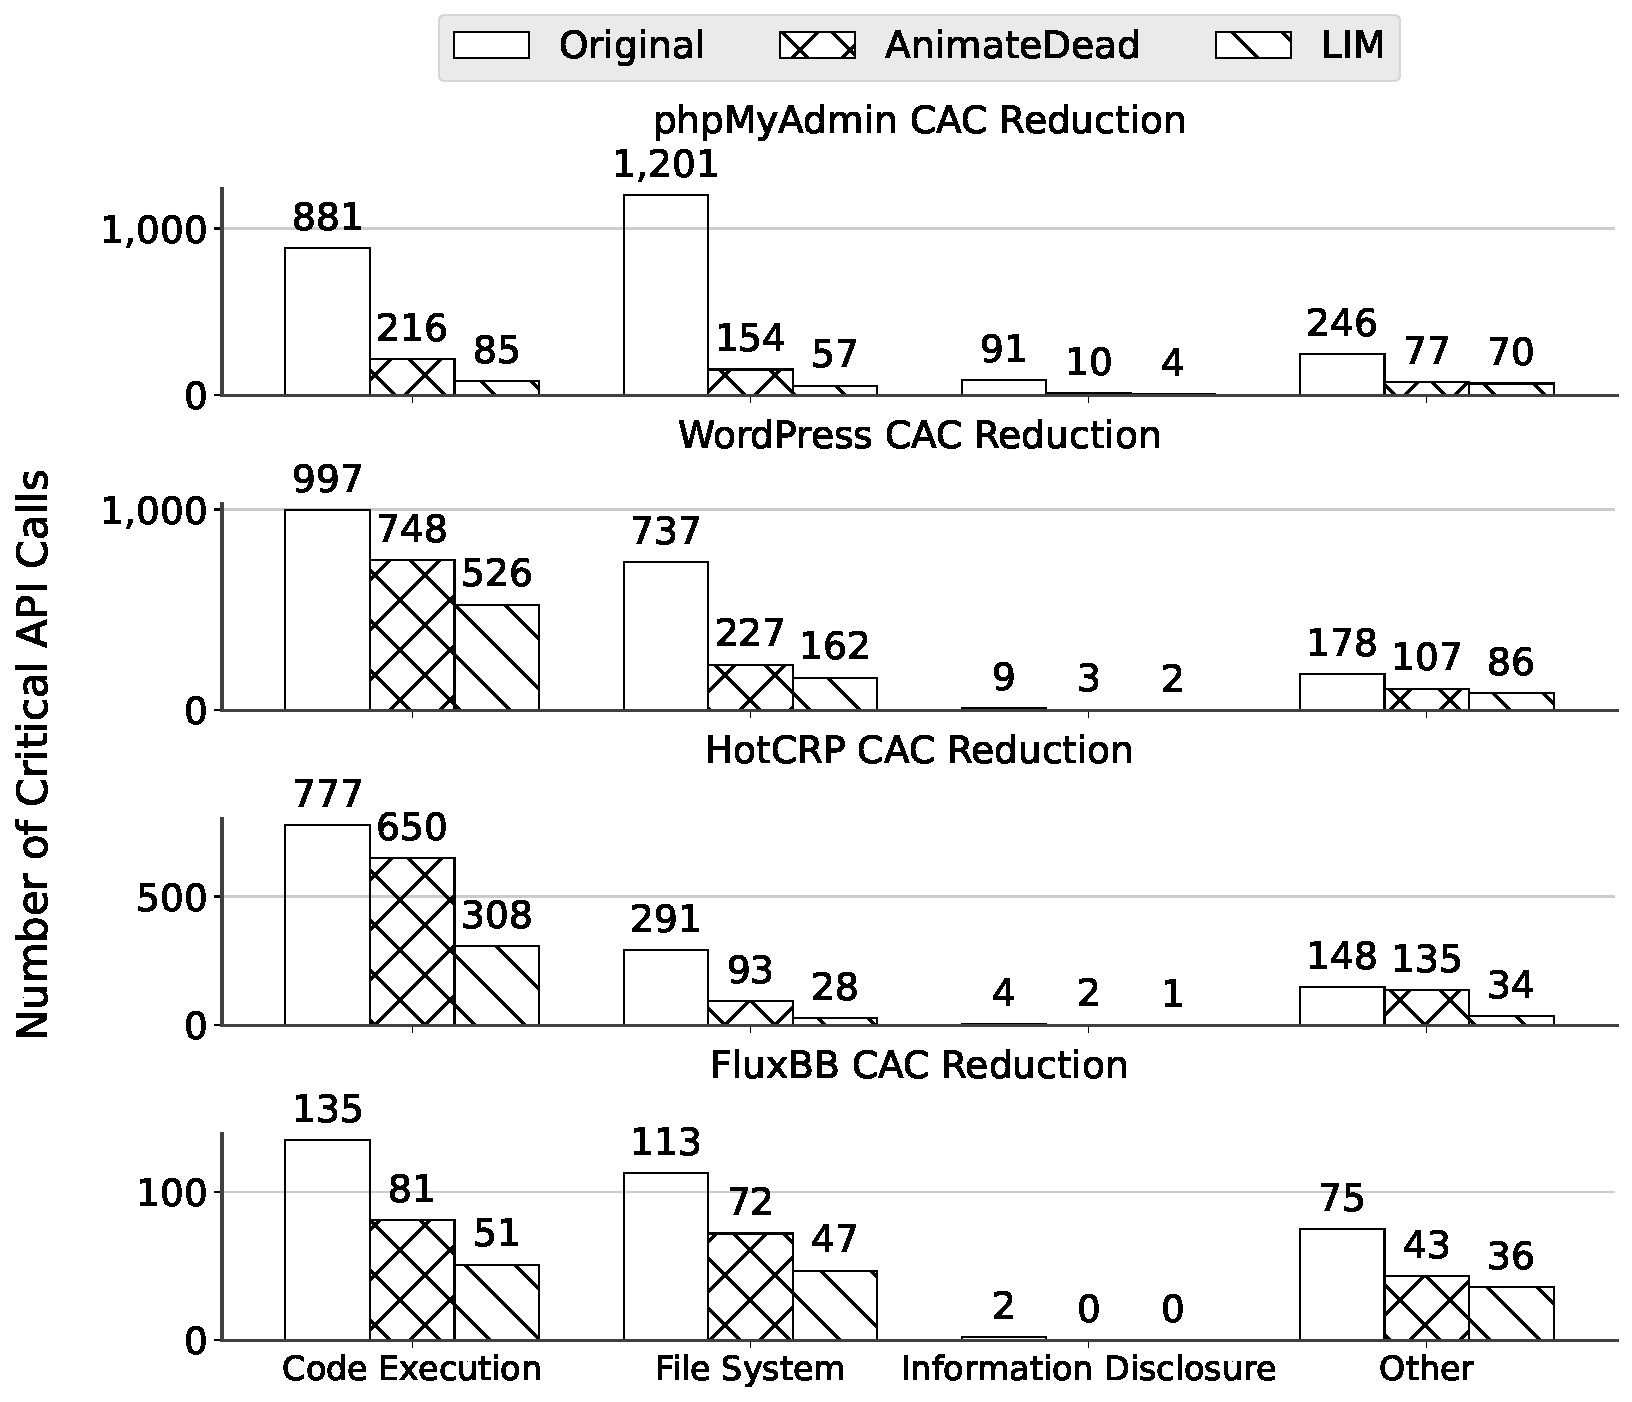
\includegraphics[width=0.8\linewidth]{figures/ad/cac_reduction_bw.pdf}
    \caption{Reduction of Critical API Calls.}
    \label{fig:cac_reduction}
\end{figure}

The PHP engine interacts with its execution environment through a set of internal APIs. 
These APIs enable web applications to interact with the file system, network or even the database. 
Similar to system calls in binary applications, abuse of Critical PHP APIs (e.g., \texttt{eval}) is closely related to the amount of damage an attacker can do. 
Previous work in the area of exploit prevention and debloating has emphasized the importance of protecting critical APIs~\cite{Mishra2018, pappas2012kbouncer, fratric2012ropguard, bulekov2021saphire}. 

We use the list of 205 critical APIs used by RIPS to perform taint analysis on PHP applications for vulnerability discovery~\cite{dahse2010rips}. 
We report the removal of these APIs after debloating. 
For phpMyAdmin, we observe that \animatedead{} removes 75\% of code execution API calls, compared to 90\% reduction of Less is More. 
For other applications in our dataset, this reduction of critical API calls ranges from 10\% to 89\% for \animatedead{} and 50\% to 96\% for Less is More. 
As demonstrated in Figure~\ref{fig:cac_reduction}, debloating based on concolic execution of entry points results in a considerable reduction in critical API calls compared to the original applications, across all categories of critical APIs. 

\subsubsection*{CVE Reduction}
Orthogonal to size reduction, we measure the performance of debloating in removing historic vulnerabilities in the source code of an application. 
To that end, for web applications present on public CVE databases (phpMyAdmin and WordPress), we reuse the CVE to source code mapping information available in the prior work~\cite{azad2019less}.

Table~\ref{tab:cve_reduction} lists the removal of CVEs after debloating. 
For both web applications, file debloating of \animatedead{} and LIM remove the same number of CVEs. 
Similarly, for WordPress, function debloating of \animatedead{} and LIM retain seven CVEs. 
For phpMyAdmin, function debloating results show that \animatedead{}'s debloating retains three CVEs more than LIM. 

We analyzed the three extra CVEs. 
For the first vulnerability (CVE-2016-5703), LIM retains multiple call sites for the vulnerable function, none of which were invoked during the dynamic tests. 
Since the path conditions for these call sites rely on database values (i.e., symbolic), \animatedead{} correctly retains the vulnerable function to preserve the correct functionality. 
Second vulnerability (CVE-2016-6633) resides in the ``import'' page of phpMyAdmin. 
Selenium tests only import SQL files while phpMyAdmin supports seven formats (e.g., zip, CSV, XML). 
Since the uploaded file format is selected by the user and is therefore symbolic, \animatedead{} retains other import formats including the one with the vulnerability. 
Lastly, we analyzed CVE-2016-6619 which resides in ``recent favorite tables'' feature, if the users request the list of recent tables without having selected any tables before, the vulnerable function would be invoked. 

The performance of \animatedead{} and LIM in the removal of CVEs for WordPress is identical. 
For the three CVEs that were removed only by LIM, we analyzed the source code of phpMyAdmin and identified that in all cases, there exists at least one symbolic code path (based on user-controlled parameters or database values) that can call the vulnerable functions, and therefore, \animatedead{} correctly retained the CVEs to preserve the correct functionality in the debloated web application. 


\subsubsection*{Removal of Object Injection Gadgets}
Improper use of deserialization APIs in PHP can lead to object injection vulnerabilities. 
This vulnerability allows attackers to build a chain of function calls through existing classes in the vulnerable web applications--known as gadget chains--to mount exploits such as SQL injection, arbitrary file write, and even remote code execution. 

Removal of gadget chains via debloating protects web applications and complicates the exploitation of object injection vulnerabilities. 
We use PHPGGC, a public repository that tracks the known gadget chains in popular web applications and third-party packages~\cite{PHPGGC}, to identify gadgets for phpMyAdmin and its third-party packages as well as WordPress. 
Their dataset does not include gadgets for HotCRP and FluxBB and therefore we only report the gadget chain reduction for phpMyAdmin and WordPress.

We identified three gadget chains for phpMyAdmin and two for WordPress.
For WordPress, both \animatedead{} and LIM successfully removed all gadget chains protecting the web application against exploits even in the presence of an object injection vulnerability. 
In the case of phpMyAdmin, one out of the three gadget chains remains in the source code after debloating via both \animatedead{} and LIM. 
This gadget belongs to the tcpdf library used by phpMyAdmin to generate PDF files. 
The gadget chain makes use of the class constructor in the main module of tcpdf (i.e., \texttt{tcpdf.php}). 
phpMyAdmin invokes the constructor of all available Export modules (including the PDF format) upon using the database export functionality and as a result, this gadget chain--correctly--remains in the debloated web applications.

\begin{table}[]
    \caption{Reduction of CVEs for phpMyAdmin and WordPress with concolic debloating of \animatedead{} and dynamic debloating of Less is More. \animatedead{} and LIM columns show the number of CVEs remaining after debloating with the specified strategy (i.e., File vs. Function debloating).}
    \label{tab:cve_reduction}
    \centering
    \begin{adjustbox}{max width=\columnwidth}
    \begin{tabular}{|l|c|cc|cc|}
    \hline
    \multirow{2}{*}{\textbf{Web Application}} & \multirow{2}{*}{\textbf{Original}} & \multicolumn{2}{c|}{\textbf{AnimateDead}}                 & \multicolumn{2}{c|}{\textbf{LIM}}    \\ \cline{3-6} 
                                              &                                    & \multicolumn{1}{c|}{File} & \multicolumn{1}{c|}{Function} & \multicolumn{1}{c|}{File} & Function \\ \hline
    phpMyAdmin                                & 20                                 & \multicolumn{1}{c|}{12}    & 7                             & \multicolumn{1}{c|}{12}    & 4        \\ \hline
    WordPress                                 & 20                                 & \multicolumn{1}{c|}{19}   & 13                             & \multicolumn{1}{c|}{19}   & 13        \\ \hline
    \end{tabular}
    \end{adjustbox}
\end{table}

\subsection{Assessment of Correctness}
In this section, we discuss the experiments that we designed to evaluate the correctness of the debloated web applications by \animatedead{}. 
We envision several categorical threats to the correctness of debloated web applications (i.e., removal of required features): 

\noindent \textbf{Implementation bugs:} 
Any flaw in the implementation of the emulator which leads to a different outcome during the execution (e.g., taking a different branch) can potentially lead to missing code-coverage. 
To address this concern, first, we created unit tests to check for the core functionality of our emulator. 
Next, we extracted code structures that handled symbolic variables from popular PHP applications in our dataset and isolated the expected behavior to verify the correct emulation results in \animatedead{}. 
Lastly, we replayed the dynamic execution traces (i.e., Selenium tests) against debloated web applications to ensure that \animatedead{}'s debloating did not break any of the previously exercised functionality.

\noindent \textbf{State space explosion:} 
Another source of missing code-coverage is rooted in the state space explosion problem. 
For larger PHP applications in our dataset (i.e., phpMyAdmin, WordPress, and HotCRP), the total number of satisfiable symbolic conditions in the applications leads to the generation of an exponentially growing number of paths for each entry point. 

As a result, exploring every single path is not feasible, nor desired particularly because the majority of explored paths do not lead to the discovery of new files and functions.  
To address this challenge, as discussed in Section~\ref{sec:path_priority}, we proposed an efficient path prioritization strategy that in practice, addressed the path explosion issue in the context of producing the correct code-coverage for applications in our dataset. 

One of the key challenges of verifying the correctness of a debloating scheme is the lack of ground truth code-coverage information. 
Dynamic code-coverage traces can be used as a lower-bound of line-coverage. 
In the absence of an oracle that determines all the reachable lines of code from each entry point given a symbolic environment we rely on automated random testing. 

\subsubsection{Automated Random testing}
\label{sec:automated_random_testing}
We use ZAP Proxy~\cite{zapproxy} and its automated crawler to interact with the same entry points used for debloating. 
By performing random testing on the same entry points used for debloating, we automatically exercise the features that are reachable from the same entry points, which should be retained by \animatedead{}. 

We execute ZAP Proxy in spider and scan mode for up to 1 hour with the authenticated session cookies and login credentials of the web applications. 
Overall, ZAP sent 86,649 requests towards the four debloated web applications in our dataset. 
We instrumented these applications to log requests towards debloating files and functions and store the entry point for those requests. 
``Errors'' column  in Table~\ref{tab:dynamic_tests} indicates the total number of unique entry points that invoked a debloated module. 
Errors are considered false positives \emph{only if} they were triggered from one of the entry points that \animatedead{} used for debloating. 
The number of reported false positives in Table~\ref{tab:dynamic_tests} refer to the number of missing files or functions and not the number of entry points. 
After a close inspection, we attribute \emph{all} the errors for \animatedead{} debloated web applications to interaction of ZAP with new entry points. 
Conversely, for web applications debloated with LIM, we identified six missing functions in phpMyAdmin related to authentication cookies, error handling, and logging. 
Similarly for WordPress, six functions from themes, cookie and session management, and failed login module were removed that triggered an error by our crawler. 
Lastly, for FluxBB, we identified two missing functions from the database adapter and password verification modules. 

The results of dynamic tests indicate that given the same entry points, dynamic debloating schemes such as LIM rely on an extensive training stage to retain all the functionality that their users need. 
In contrast, concolic execution in \animatedead{} performs its analysis based on abstract inputs (e.g., correct and incorrect login credentials) and as a result, provides more robust debloated applications without relying on server side instrumentation and extensive training data. 

\begin{table}[]
    \caption{Automated random testing results including the total number of requests made by ZAP Proxy crawler, number of entry points that triggered an error and number of missing files or functions that triggered false positives (i.e., requests towards entry points from the logs that invoked a debloated module)}
    \label{tab:dynamic_tests}
    \centering
    \begin{adjustbox}{max width=\columnwidth}
    \begin{tabular}{|l|c|c|cc|}
        \hline
        \multirow{2}{*}{\textbf{Web Application}} & \multirow{2}{*}{\textbf{Requests}} & \multirow{2}{*}{\textbf{Errors}} & \multicolumn{2}{c|}{\textbf{False Positives}}               \\ \cline{4-5} 
                                                  &                                    &                                  & \multicolumn{1}{l|}{AnimateDead} & \multicolumn{1}{l|}{LIM} \\ \hline
        phpMyAdmin                                & 21,040                             & 6                                & \multicolumn{1}{c|}{0}           & 6                        \\ \hline
        WordPress                                 & 31,055                             & 102                              & \multicolumn{1}{c|}{0}           & 6                        \\ \hline
        HotCRP                                    & 16,021                             & 12                               & \multicolumn{1}{c|}{0}           & 0                        \\ \hline
        FluxBB                                    & 18,533                             & 3                                & \multicolumn{1}{c|}{0}           & 2                        \\ \hline
        \end{tabular}
    \end{adjustbox}
\end{table}